\begin{frame}{Conclusion}
	Il est possible de quantifier la pertinence des termes scientifiques partagés entre Charcot et son réseau
	\bigskip
	
	\danger Limitations de l'approche linguistique de l'extraction des termes\\$\rightarrow$ les termes plus pointus sont pénalisés
			
\bigskip
	À faire :
	\begin{itemize}
		\item rendre compte du contexte d'énonciation des termes
		\item déterminer l'approche à adopter (plongements dynamiques ? )
		\item trouver un corpus \og{}externe\fg{} : prouver la pertinence des termes détectés pour la communauté scientifique
%		\item concevoir une approche spécifique qui permette de gérer soigneusement la collection de documents, le dictionnaire de termes, ou les deux
%		\item choisir des termes spécifiques et expliquer le contexte historique, ses différentes étapes et la signification que ces termes ont pour un groupe spécifique d'experts
	\end{itemize}
\end{frame}

%\begin{frame}{Évolution du projet}
%\begin{figure}[h]
%    \centering
%    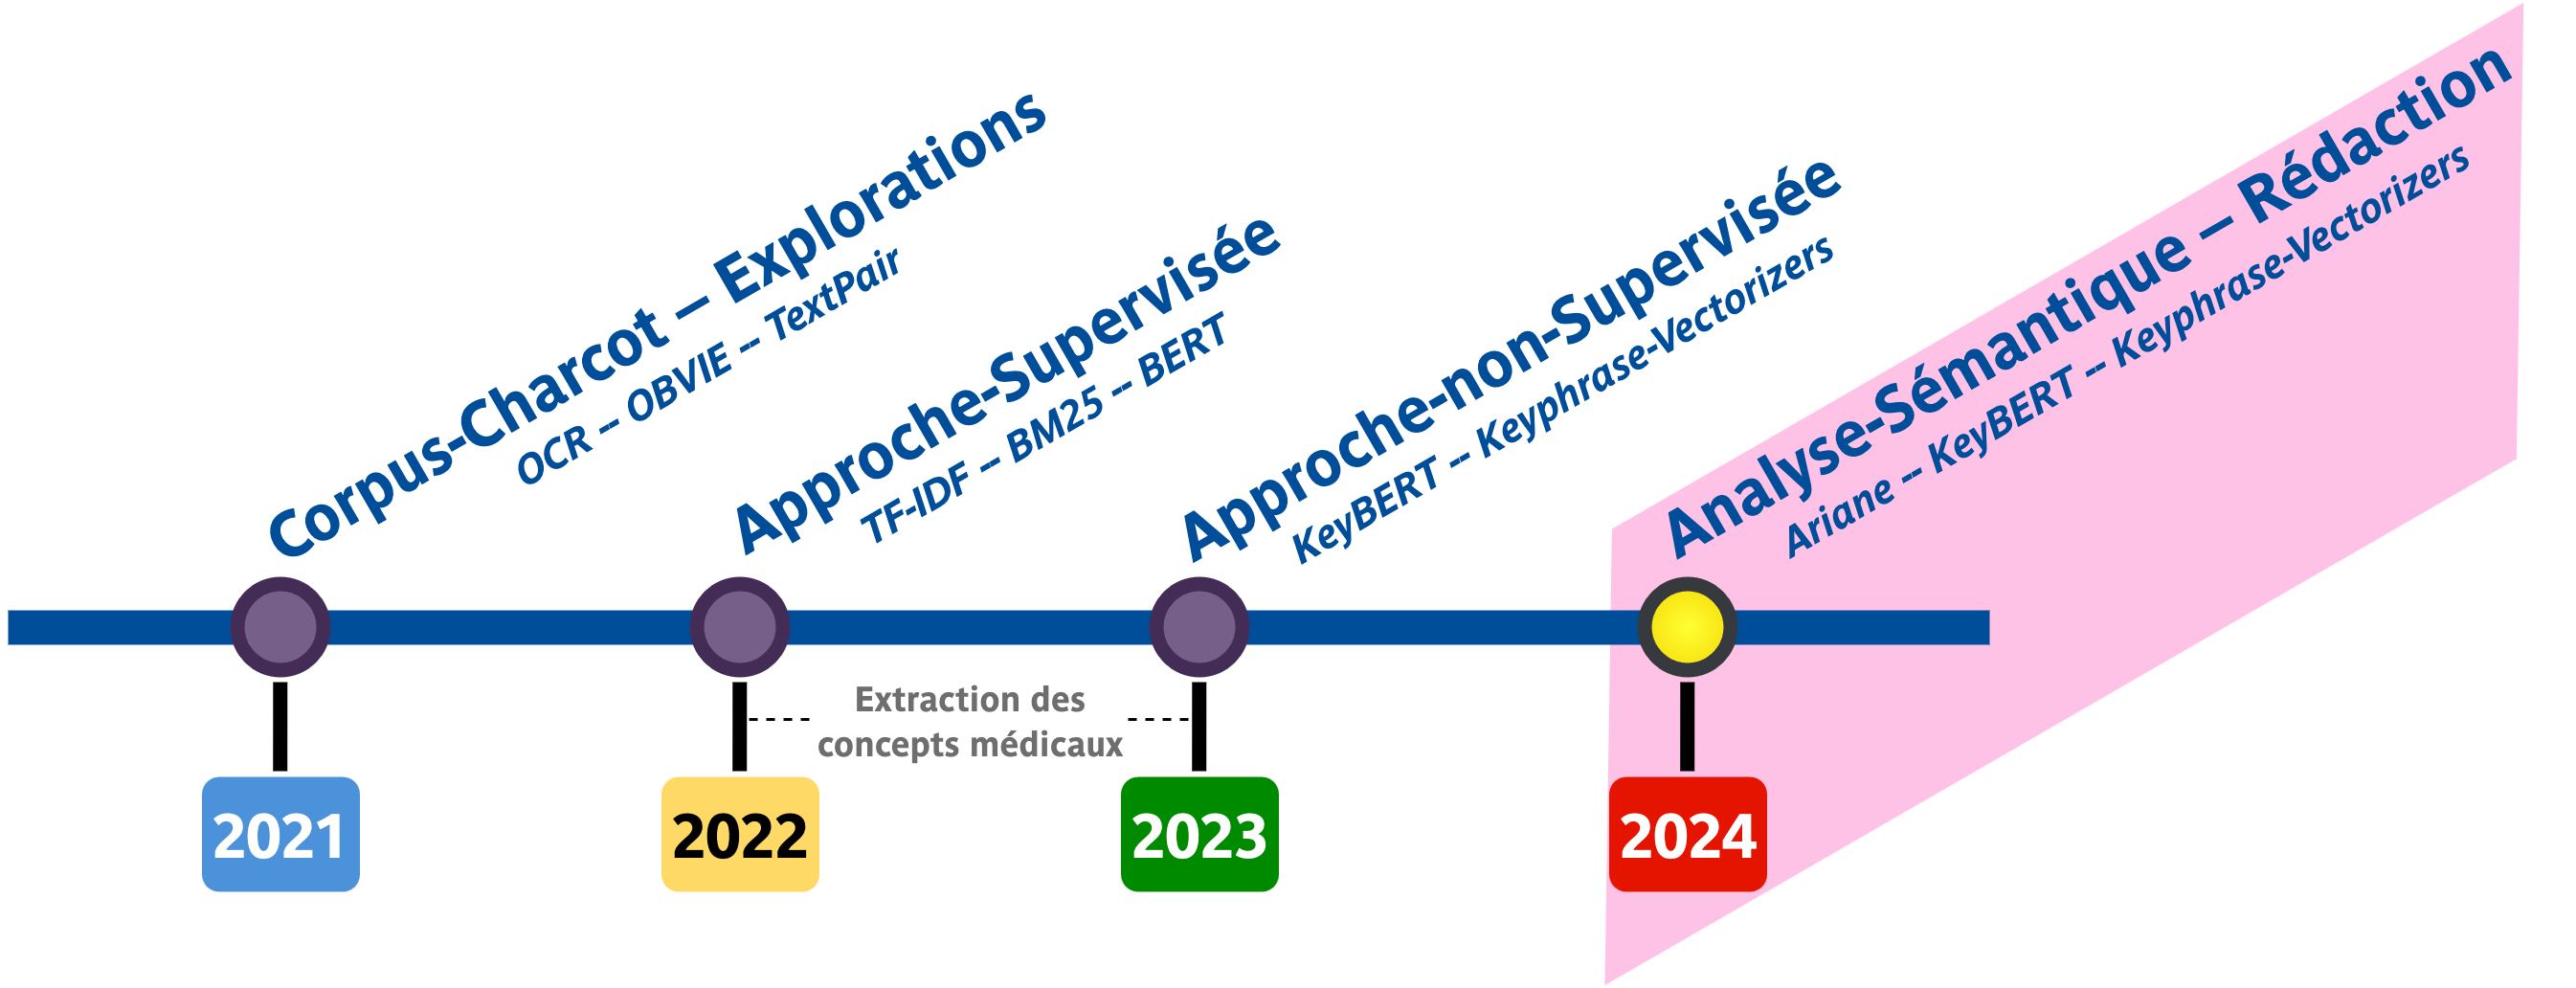
\includegraphics[width=1\textwidth]{pic/timeline_Charcot.png}
%    \label{fig:enter-label}
%    \caption{Méthodes computationnelles déjà expérimentées et à expérimenter.}
%\end{figure}
%$\rightarrow$ histoire des concepts {\footnotesize(allem. \textit{Begriffsgeschichte}) \citep{koselleck2011introduction}}
%\end{frame}